\documentclass{standalone}
\usepackage{tikz}
\usetikzlibrary{patterns, positioning}
\usepackage[sfdefault]{ClearSans} %% option 'sfdefault' activates Clear Sans as the default text font
\usepackage[T1]{fontenc}

\begin{document}
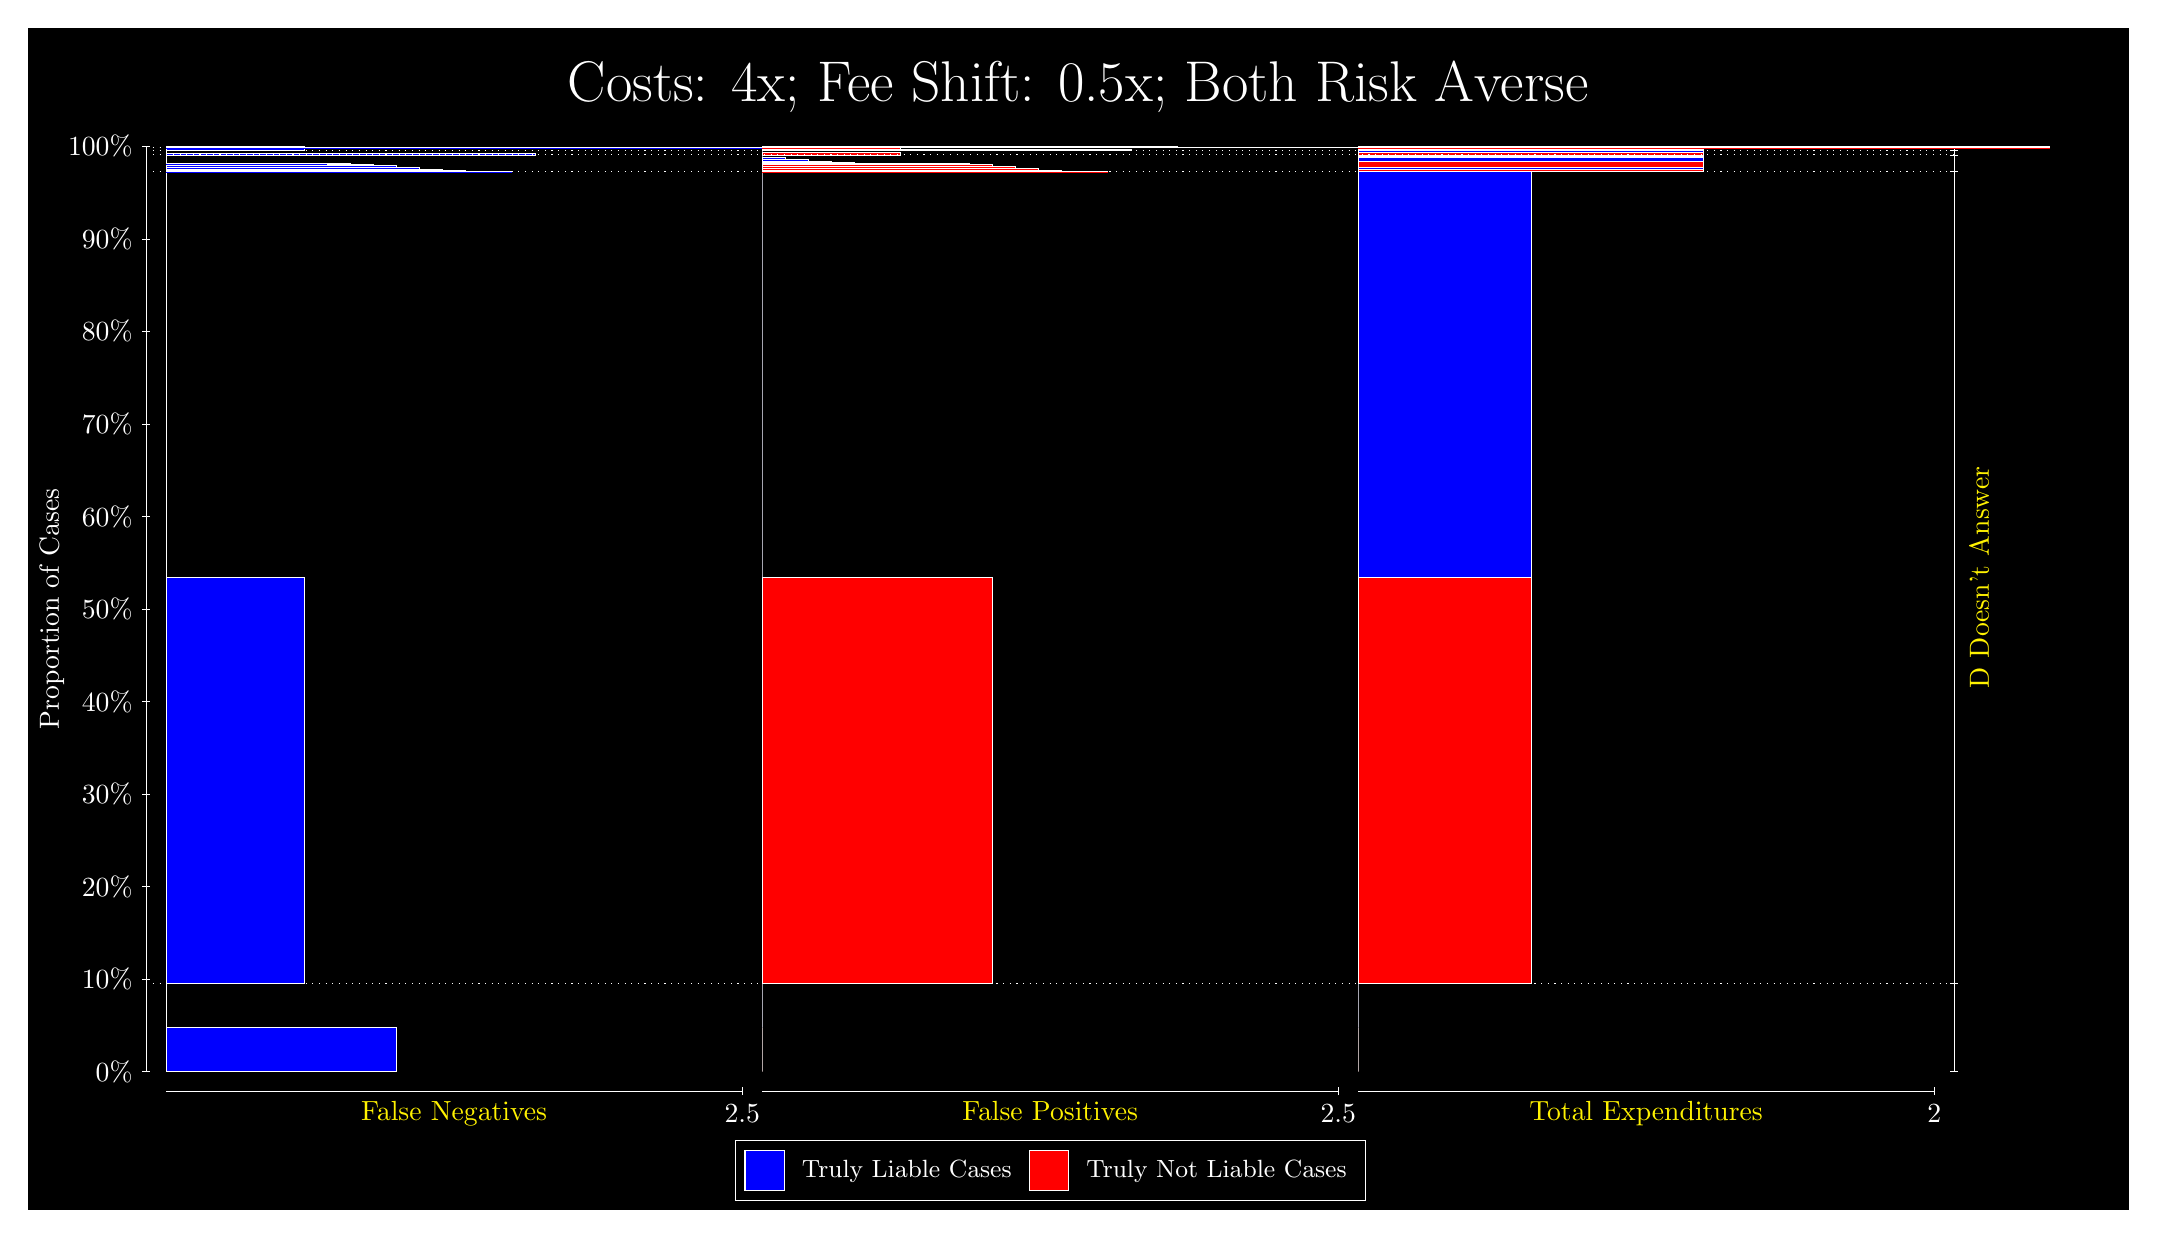
\begin{tikzpicture}
\draw[fill=black] (0,0) rectangle (26.667,15);
\draw[text=white] (0,13.5) rectangle (26.667,15) node[midway] {\huge Costs: 4x; Fee Shift: 0.5x; Both Risk Averse};
\draw[white, very thin] (1.5,1.75) -- (1.5,13.5);
\node[rotate=90, text=white, anchor=center] at (0.3, 7.625) {Proportion of Cases};
\draw[white, very thin] (1.45,1.75) -- (1.55,1.75);
\node[text=white, anchor=east] at (1.45, 1.75) {0\%};
\draw[white, very thin] (1.45,2.925) -- (1.55,2.925);
\node[text=white, anchor=east] at (1.45, 2.925) {10\%};
\draw[white, very thin] (1.45,4.1) -- (1.55,4.1);
\node[text=white, anchor=east] at (1.45, 4.1) {20\%};
\draw[white, very thin] (1.45,5.275) -- (1.55,5.275);
\node[text=white, anchor=east] at (1.45, 5.275) {30\%};
\draw[white, very thin] (1.45,6.45) -- (1.55,6.45);
\node[text=white, anchor=east] at (1.45, 6.45) {40\%};
\draw[white, very thin] (1.45,7.625) -- (1.55,7.625);
\node[text=white, anchor=east] at (1.45, 7.625) {50\%};
\draw[white, very thin] (1.45,8.8) -- (1.55,8.8);
\node[text=white, anchor=east] at (1.45, 8.8) {60\%};
\draw[white, very thin] (1.45,9.975) -- (1.55,9.975);
\node[text=white, anchor=east] at (1.45, 9.975) {70\%};
\draw[white, very thin] (1.45,11.15) -- (1.55,11.15);
\node[text=white, anchor=east] at (1.45, 11.15) {80\%};
\draw[white, very thin] (1.45,12.325) -- (1.55,12.325);
\node[text=white, anchor=east] at (1.45, 12.325) {90\%};
\draw[white, very thin] (1.45,13.5) -- (1.55,13.5);
\node[text=white, anchor=east] at (1.45, 13.5) {100\%};

\draw[white, very thin] (24.457,1.75) -- (24.457,13.5);
\draw[white, very thin] (24.407,1.75) -- (24.507,1.75);
\node[anchor=west] at (24.407, 1.75) {};
\draw[white, very thin] (24.407,2.8673) -- (24.507,2.8673);
\node[anchor=west] at (24.407, 2.8673) {};
\draw[white, very thin] (24.407,13.179) -- (24.507,13.179);
\node[anchor=west] at (24.407, 13.179) {};
\draw[white, very thin] (24.407,13.392) -- (24.507,13.392);
\node[anchor=west] at (24.407, 13.392) {};
\draw[white, very thin] (24.407,13.45) -- (24.507,13.45);
\node[anchor=west] at (24.407, 13.45) {};
\draw[white, very thin] (24.407,13.483) -- (24.507,13.483);
\node[anchor=west] at (24.407, 13.483) {};
\draw[white, very thin] (24.407,13.486) -- (24.507,13.486);
\node[anchor=west] at (24.407, 13.486) {};
\draw[white, very thin] (24.407,13.5) -- (24.507,13.5);
\node[anchor=west] at (24.407, 13.5) {};

\draw[white, very thin, fill=blue] (1.75,1.75) rectangle (4.6775,2.3087);
\draw[white, very thin, fill=red] (1.75,2.3087) rectangle (1.75,2.8673);
\draw[white, very thin, fill=blue] (1.75,2.8673) rectangle (3.5065,8.0245);
\draw[white, very thin, fill=red] (1.75,8.0245) rectangle (1.75,13.179);
\draw[white, very thin, fill=blue] (1.75,13.179) rectangle (6.1413,13.18);
\draw[white, very thin, fill=blue] (1.75,13.18) rectangle (5.8486,13.182);
\draw[white, very thin, fill=blue] (1.75,13.182) rectangle (5.5558,13.195);
\draw[white, very thin, fill=blue] (1.75,13.195) rectangle (5.2631,13.21);
\draw[white, very thin, fill=blue] (1.75,13.21) rectangle (4.9703,13.237);
\draw[white, very thin, fill=blue] (1.75,13.237) rectangle (4.6775,13.261);
\draw[white, very thin, fill=blue] (1.75,13.261) rectangle (4.3848,13.276);
\draw[white, very thin, fill=blue] (1.75,13.276) rectangle (4.092,13.279);
\draw[white, very thin, fill=blue] (1.75,13.279) rectangle (3.7993,13.281);
\draw[white, very thin, fill=red] (1.75,13.281) rectangle (1.75,13.392);
\draw[white, very thin, fill=blue] (1.75,13.392) rectangle (6.4341,13.416);
\draw[white, very thin, fill=red] (1.75,13.416) rectangle (1.75,13.45);
\draw[white, very thin, fill=blue] (1.75,13.45) rectangle (3.5065,13.47);
\draw[white, very thin, fill=red] (1.75,13.47) rectangle (1.75,13.483);
\draw[white, very thin, fill=blue] (1.75,13.483) rectangle (9.9471,13.485);
\draw[white, very thin, fill=red] (1.75,13.485) rectangle (1.75,13.486);
\draw[white, very thin, fill=blue] (1.75,13.486) rectangle (3.5065,13.498);
\draw[white, very thin, fill=red] (1.75,13.498) rectangle (1.75,13.5);
\draw[white, very thin, fill=red] (9.3189,1.75) rectangle (9.3189,2.3087);
\draw[white, very thin, fill=blue] (9.3189,2.3087) rectangle (9.3189,2.8673);
\draw[white, very thin, fill=red] (9.3189,2.8673) rectangle (12.246,8.022);
\draw[white, very thin, fill=blue] (9.3189,8.022) rectangle (9.3189,13.179);
\draw[white, very thin, fill=red] (9.3189,13.179) rectangle (13.71,13.18);
\draw[white, very thin, fill=red] (9.3189,13.18) rectangle (13.417,13.181);
\draw[white, very thin, fill=red] (9.3189,13.181) rectangle (13.125,13.194);
\draw[white, very thin, fill=red] (9.3189,13.194) rectangle (12.832,13.221);
\draw[white, very thin, fill=red] (9.3189,13.221) rectangle (12.539,13.251);
\draw[white, very thin, fill=red] (9.3189,13.251) rectangle (12.246,13.27);
\draw[white, very thin, fill=red] (9.3189,13.27) rectangle (11.954,13.288);
\draw[white, very thin, fill=red] (9.3189,13.288) rectangle (11.661,13.289);
\draw[white, very thin, fill=red] (9.3189,13.289) rectangle (11.368,13.29);
\draw[white, very thin, fill=blue] (9.3189,13.29) rectangle (10.783,13.291);
\draw[white, very thin, fill=blue] (9.3189,13.291) rectangle (10.49,13.294);
\draw[white, very thin, fill=blue] (9.3189,13.294) rectangle (10.197,13.31);
\draw[white, very thin, fill=blue] (9.3189,13.31) rectangle (9.9044,13.334);
\draw[white, very thin, fill=blue] (9.3189,13.334) rectangle (9.6116,13.361);
\draw[white, very thin, fill=blue] (9.3189,13.361) rectangle (9.3189,13.392);
\draw[white, very thin, fill=red] (9.3189,13.392) rectangle (11.075,13.426);
\draw[white, very thin, fill=blue] (9.3189,13.426) rectangle (9.3189,13.45);
\draw[white, very thin, fill=red] (9.3189,13.45) rectangle (14.003,13.464);
\draw[white, very thin, fill=blue] (9.3189,13.464) rectangle (11.075,13.483);
\draw[white, very thin, fill=red] (9.3189,13.483) rectangle (11.075,13.485);
\draw[white, very thin, fill=blue] (9.3189,13.485) rectangle (9.3189,13.486);
\draw[white, very thin, fill=red] (9.3189,13.486) rectangle (17.516,13.488);
\draw[white, very thin, fill=blue] (9.3189,13.488) rectangle (14.588,13.5);
\draw[white, very thin, fill=red] (16.888,1.75) rectangle (16.888,2.3087);
\draw[white, very thin, fill=blue] (16.888,2.3087) rectangle (16.888,2.8673);
\draw[white, very thin, fill=red] (16.888,2.8673) rectangle (19.083,8.022);
\draw[white, very thin, fill=blue] (16.888,8.022) rectangle (19.083,13.179);
\draw[white, very thin, fill=red] (16.888,13.179) rectangle (21.279,13.209);
\draw[white, very thin, fill=blue] (16.888,13.209) rectangle (21.279,13.236);
\draw[white, very thin, fill=red] (16.888,13.236) rectangle (21.279,13.304);
\draw[white, very thin, fill=blue] (16.888,13.304) rectangle (21.279,13.36);
\draw[white, very thin, fill=red] (16.888,13.36) rectangle (21.279,13.373);
\draw[white, very thin, fill=blue] (16.888,13.373) rectangle (21.279,13.392);
\draw[white, very thin, fill=red] (16.888,13.392) rectangle (21.279,13.426);
\draw[white, very thin, fill=blue] (16.888,13.426) rectangle (21.279,13.45);
\draw[white, very thin, fill=red] (16.888,13.45) rectangle (21.279,13.464);
\draw[white, very thin, fill=blue] (16.888,13.464) rectangle (21.279,13.483);
\draw[white, very thin, fill=red] (16.888,13.483) rectangle (25.67,13.485);
\draw[white, very thin, fill=blue] (16.888,13.485) rectangle (25.67,13.486);
\draw[white, very thin, fill=red] (16.888,13.486) rectangle (25.67,13.488);
\draw[white, very thin, fill=blue] (16.888,13.488) rectangle (25.67,13.5);
\draw[white, dotted] (1.5,2.8673) -- (24.457,2.8673);
\draw[white, dotted] (1.5,13.179) -- (24.457,13.179);
\draw[white, dotted] (1.5,13.392) -- (24.457,13.392);
\draw[white, dotted] (1.5,13.45) -- (24.457,13.45);
\draw[white, dotted] (1.5,13.483) -- (24.457,13.483);
\draw[white, dotted] (1.5,13.486) -- (24.457,13.486);
\draw[white, very thin] (1.75,1.5) -- (9.0689,1.5);
\node[text=yellow, anchor=north] at (5.4094, 1.5) {False Negatives};
\draw[white, very thin] (9.0689,1.45) -- (9.0689,1.55);
\node[text=white, anchor=north] at (9.0689, 1.45) {2.5};

\draw[white, very thin] (9.3189,1.5) -- (16.638,1.5);
\node[text=yellow, anchor=north] at (12.978, 1.5) {False Positives};
\draw[white, very thin] (16.638,1.45) -- (16.638,1.55);
\node[text=white, anchor=north] at (16.638, 1.45) {2.5};

\draw[white, very thin] (16.888,1.5) -- (24.207,1.5);
\node[text=yellow, anchor=north] at (20.547, 1.5) {Total Expenditures};
\draw[white, very thin] (24.207,1.45) -- (24.207,1.55);
\node[text=white, anchor=north] at (24.207, 1.45) {2};


\node[text=yellow, centered, rotate=90] at (24.777, 8.0232) {D Doesn't Answer};






\draw (12.978300999999998,1.5) node[draw=none] (baseCoordinate) {};
\begin{scope}[align=center]
        \matrix[scale=0.5, draw=white, below=0.5cm of baseCoordinate, nodes={draw}, column sep=0.1cm]{
            \node[rectangle, draw, minimum width=0.5cm, minimum height=0.5cm, fill=blue] {}; &
            \node[draw=none, font=\small, text=white] (B) {Truly Liable Cases}; &
            \node[rectangle, draw, minimum width=0.5cm, minimum height=0.5cm, fill=red] {}; &
            \node[draw=none, font=\small, text=white] (B) {Truly Not Liable Cases}; \\
            };
\end{scope}

\end{tikzpicture}
\end{document}